\chapter{El Centro de Alto Rendimiento Computacional ZINE}
\label{chap:zine}

Este capítulo describe el Centro de Alto Rendimiento Computacional Javeriano (ZINE), abordando su origen, propósito institucional y el conjunto de servicios que ofrece tanto a la comunidad universitaria como a usuarios externos, en el marco del uso científico y académico de la computación de alto rendimiento.

\begin{figure}[h]
  \centering
  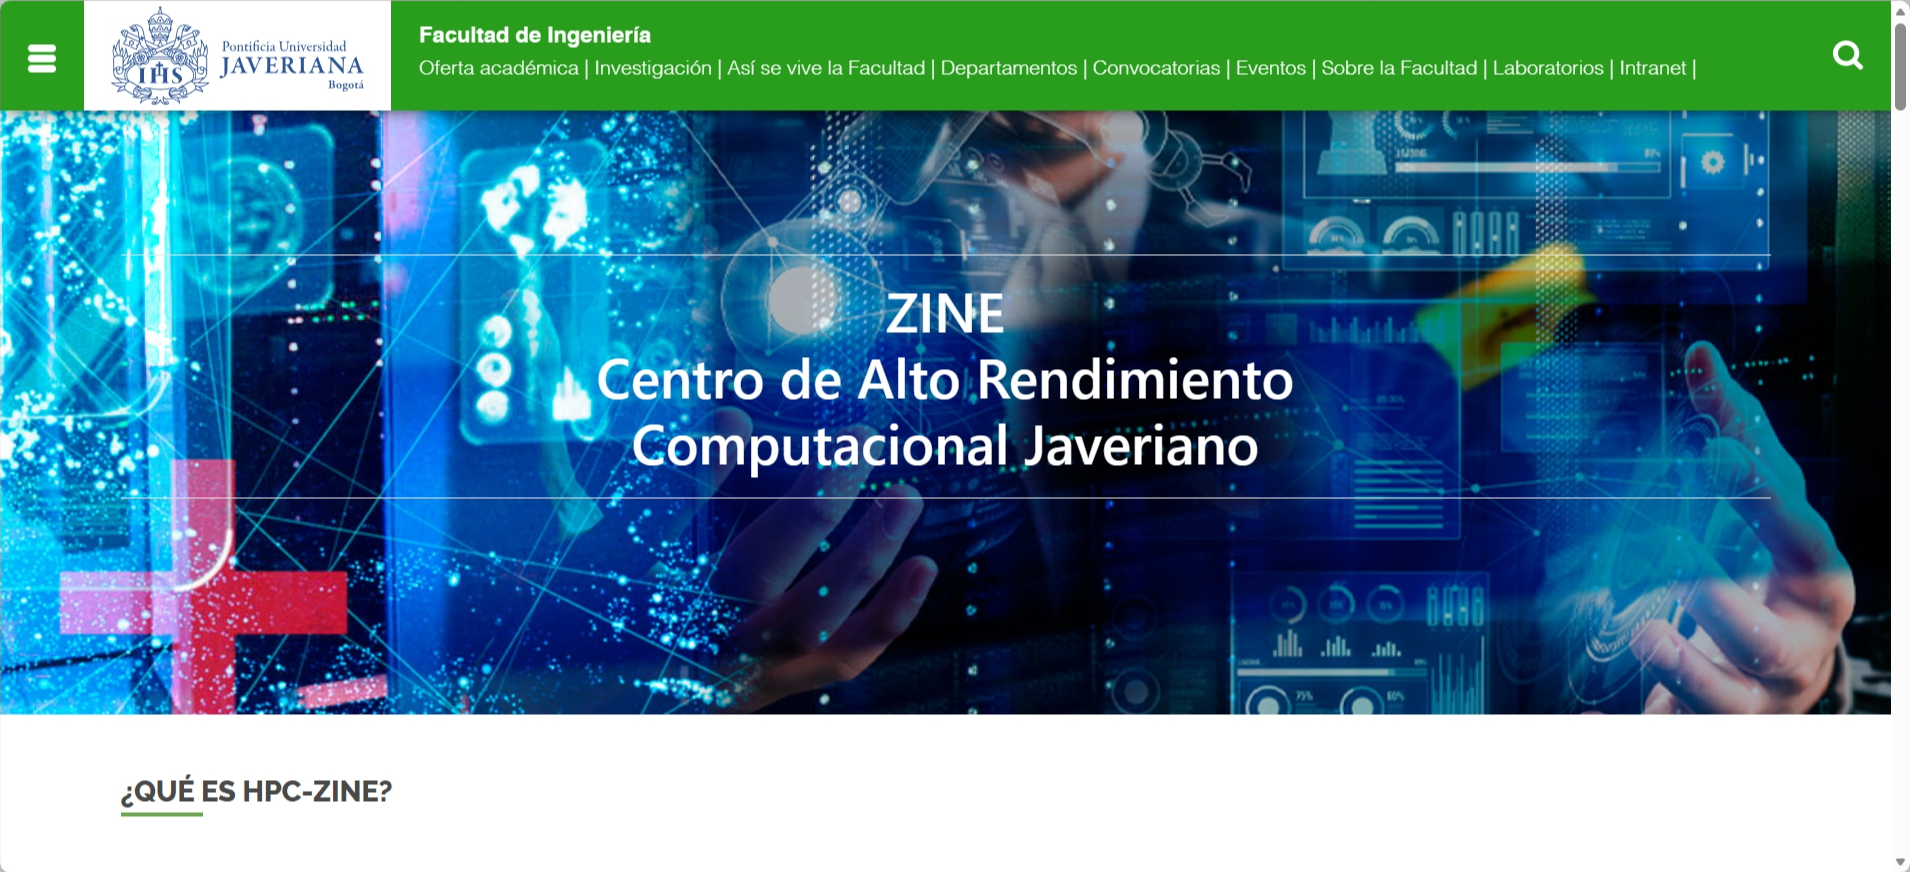
\includegraphics[width=0.95\textwidth]{images/ZINE/zine_pagina_oficial.png}
  \caption{Página oficial del Centro de Alto Rendimiento Computacional ZINE.\\Para mas información visite la web oficial https://ingenieria.javeriana.edu.co/zine}
  \label{fig:zine_web}
\end{figure}

\section{¿Por qué nace ZINE?}
La investigación científica contemporánea plantea problemas cuyo tamaño, complejidad o volumen de datos hacen inviable su ejecución eficiente en computadores convencionales. Entre estos se encuentran simulaciones numéricas, análisis intensivos de datos y modelado de sistemas complejos, como escenarios climáticos, fenómenos físicos, análisis de series de tiempo o procesamiento masivo de información. En este contexto, la computación de alto rendimiento (High Performance Computing, HPC) permite reducir significativamente los tiempos de cálculo mediante la distribución del trabajo entre múltiples procesadores y recursos especializados \cite{pesquisa_zine_2012}.

ZINE surge como respuesta a esta necesidad transversal, con el objetivo de proporcionar a investigadores de diversas disciplinas una infraestructura capaz de soportar simulaciones y análisis que demandan alta capacidad de cómputo y almacenamiento. Según la descripción institucional, su creación se originó en los requerimientos de investigadores que necesitan simular y analizar grandes volúmenes de datos, y su infraestructura se encuentra alojada en el Datacenter de la Universidad, lo que garantiza continuidad y disponibilidad del servicio \cite{zine_oficial}.

Adicionalmente, ZINE fue concebido como una iniciativa orientada a fomentar la cooperación entre investigadores y grupos, tanto internos como externos, alrededor del uso de la supercomputación y tecnologías asociadas, promoviendo la adopción del HPC como herramienta fundamental para la investigación científica \cite{zine_oficial}.

\section{¿Para qué es ZINE?}
ZINE es un servicio académico y científico cuyo propósito es apoyar la investigación y la docencia mediante la provisión de capacidad de procesamiento y almacenamiento de información. Su misión institucional se define como la oferta de servicios computacionales que respaldan procesos académicos de investigación y formación \cite{zine_oficial}.

En términos operativos, ZINE permite:
\begin{itemize}
  \item \textbf{Acelerar cálculos complejos:} reducir los tiempos de ejecución de simulaciones y análisis computacionalmente intensivos.
  \item \textbf{Habilitar trabajos de gran escala:} ejecutar procesos que exceden las capacidades de equipos personales, ya sea por volumen de datos, duración o requerimientos de cómputo.
  \item \textbf{Acompañar a los usuarios:} ofrecer formación y asesoría para el uso adecuado de la infraestructura.
  \item \textbf{Fomentar la colaboración:} articular capacidades técnicas con necesidades de diferentes áreas del conocimiento.
\end{itemize}

La plataforma está orientada a soportar trabajos asociados con Big Data, Machine Learning e Inteligencia Artificial, así como otros problemas que requieren la modelación o simulación de escenarios complejos \cite{perfiles_capacidades_zine}.

\section{Servicios internos del ZINE en la Universidad Javeriana}
De acuerdo con la caracterización institucional, ZINE pone a disposición de investigadores, docentes y estudiantes una infraestructura tecnológica destinada a la ejecución de trabajos de alto volumen, así como al apoyo de procesos de simulación y análisis en múltiples áreas del conocimiento \cite{perfiles_capacidades_zine}.

Para la comunidad Javeriana, los servicios se estructuran principalmente en los siguientes componentes:

\subsection*{1) Infraestructura de cómputo y almacenamiento}
ZINE ofrece recursos computacionales y de almacenamiento diseñados para soportar cargas de trabajo intensivas, orientadas a tareas de simulación, análisis y procesamiento de grandes volúmenes de datos \cite{zine_oficial,perfiles_capacidades_zine}.

\subsection*{2) Aplicación en diversas disciplinas}
La infraestructura es utilizada para modelar y simular distintos tipos de escenarios, entre ellos:
\begin{itemize}
  \item \textbf{Escenarios físicos:} simulación del estado del tiempo y análisis de estructuras mecánicas.
  \item \textbf{Escenarios biológicos:} análisis de secuencias genéticas y fenómenos propios de las ciencias de la vida.
  \item \textbf{Escenarios económicos y de datos:} análisis de series de tiempo y problemas de ciencia de datos e ingeniería.
\end{itemize}
\cite{perfiles_capacidades_zine}

\subsection*{3) Capacitación en el uso de plataformas HPC}
Dado que el aprovechamiento efectivo de estas infraestructuras requiere conocimientos técnicos específicos, ZINE enfatiza la formación de sus usuarios. Como parte de esta estrategia, se ofrecen cursos orientados al acceso a la plataforma, el uso de gestores de tareas (por ejemplo, HTCondor) y el envío y control de trabajos computacionales \cite{curso_hpc_python}.

\subsection*{4) Acompañamiento y asesoría técnica}
Además del acceso a la infraestructura, ZINE proporciona acompañamiento técnico a los investigadores, con el fin de facilitar el uso eficiente de los recursos en sus proyectos académicos y científicos \cite{perfiles_capacidades_zine,pesquisa_zine_2012}.

\section{Servicios a investigadores externos}
ZINE extiende sus servicios más allá de la comunidad universitaria. De acuerdo con la información institucional, entidades externas pueden acceder a la infraestructura para realizar análisis y simulaciones que involucren grandes volúmenes de datos o el entrenamiento extensivo de modelos de aprendizaje automático, entre otros usos \cite{zine_oficial}.

En el portafolio de servicios externos de la Facultad de Ingeniería, ZINE se presenta como una solución de cómputo de alto desempeño que ofrece recursos computacionales, capacitación y acompañamiento para proyectos de investigación, docencia, análisis y simulación, tanto para el sector académico como para el productivo \cite{servicios_externos_zine}.

De manera concreta, para usuarios externos se contemplan líneas de servicio como:
\begin{itemize}
  \item Capacitación para el uso adecuado de infraestructura HPC.
  \item Asesoría en el despliegue de herramientas de analítica de datos e inteligencia artificial sobre plataformas de alto rendimiento.
  \item Uso de infraestructura alojada en Datacenter, con niveles de disponibilidad asociados a estándares Tier 2/3.
  \item Almacenamiento de grandes volúmenes de información, con énfasis en la soberanía y gestión responsable de los datos.
\end{itemize}
\cite{servicios_externos_zine}

Finalmente, desde una perspectiva de colaboración académica, se ha señalado que, mediante proyectos interinstitucionales, investigadores y docentes de otras universidades pueden beneficiarse del acceso a este tipo de infraestructura de cómputo avanzado \cite{pesquisa_zine_2012}.
